% Options for packages loaded elsewhere
\PassOptionsToPackage{unicode}{hyperref}
\PassOptionsToPackage{hyphens}{url}
\PassOptionsToPackage{dvipsnames,svgnames,x11names}{xcolor}
%
\documentclass[
  letterpaper,
  DIV=11,
  numbers=noendperiod]{scrartcl}

\usepackage{amsmath,amssymb}
\usepackage{lmodern}
\usepackage{iftex}
\ifPDFTeX
  \usepackage[T1]{fontenc}
  \usepackage[utf8]{inputenc}
  \usepackage{textcomp} % provide euro and other symbols
\else % if luatex or xetex
  \usepackage{unicode-math}
  \defaultfontfeatures{Scale=MatchLowercase}
  \defaultfontfeatures[\rmfamily]{Ligatures=TeX,Scale=1}
\fi
% Use upquote if available, for straight quotes in verbatim environments
\IfFileExists{upquote.sty}{\usepackage{upquote}}{}
\IfFileExists{microtype.sty}{% use microtype if available
  \usepackage[]{microtype}
  \UseMicrotypeSet[protrusion]{basicmath} % disable protrusion for tt fonts
}{}
\makeatletter
\@ifundefined{KOMAClassName}{% if non-KOMA class
  \IfFileExists{parskip.sty}{%
    \usepackage{parskip}
  }{% else
    \setlength{\parindent}{0pt}
    \setlength{\parskip}{6pt plus 2pt minus 1pt}}
}{% if KOMA class
  \KOMAoptions{parskip=half}}
\makeatother
\usepackage{xcolor}
\setlength{\emergencystretch}{3em} % prevent overfull lines
\setcounter{secnumdepth}{-\maxdimen} % remove section numbering
% Make \paragraph and \subparagraph free-standing
\ifx\paragraph\undefined\else
  \let\oldparagraph\paragraph
  \renewcommand{\paragraph}[1]{\oldparagraph{#1}\mbox{}}
\fi
\ifx\subparagraph\undefined\else
  \let\oldsubparagraph\subparagraph
  \renewcommand{\subparagraph}[1]{\oldsubparagraph{#1}\mbox{}}
\fi

\usepackage{color}
\usepackage{fancyvrb}
\newcommand{\VerbBar}{|}
\newcommand{\VERB}{\Verb[commandchars=\\\{\}]}
\DefineVerbatimEnvironment{Highlighting}{Verbatim}{commandchars=\\\{\}}
% Add ',fontsize=\small' for more characters per line
\usepackage{framed}
\definecolor{shadecolor}{RGB}{241,243,245}
\newenvironment{Shaded}{\begin{snugshade}}{\end{snugshade}}
\newcommand{\AlertTok}[1]{\textcolor[rgb]{0.68,0.00,0.00}{#1}}
\newcommand{\AnnotationTok}[1]{\textcolor[rgb]{0.37,0.37,0.37}{#1}}
\newcommand{\AttributeTok}[1]{\textcolor[rgb]{0.40,0.45,0.13}{#1}}
\newcommand{\BaseNTok}[1]{\textcolor[rgb]{0.68,0.00,0.00}{#1}}
\newcommand{\BuiltInTok}[1]{\textcolor[rgb]{0.00,0.23,0.31}{#1}}
\newcommand{\CharTok}[1]{\textcolor[rgb]{0.13,0.47,0.30}{#1}}
\newcommand{\CommentTok}[1]{\textcolor[rgb]{0.37,0.37,0.37}{#1}}
\newcommand{\CommentVarTok}[1]{\textcolor[rgb]{0.37,0.37,0.37}{\textit{#1}}}
\newcommand{\ConstantTok}[1]{\textcolor[rgb]{0.56,0.35,0.01}{#1}}
\newcommand{\ControlFlowTok}[1]{\textcolor[rgb]{0.00,0.23,0.31}{#1}}
\newcommand{\DataTypeTok}[1]{\textcolor[rgb]{0.68,0.00,0.00}{#1}}
\newcommand{\DecValTok}[1]{\textcolor[rgb]{0.68,0.00,0.00}{#1}}
\newcommand{\DocumentationTok}[1]{\textcolor[rgb]{0.37,0.37,0.37}{\textit{#1}}}
\newcommand{\ErrorTok}[1]{\textcolor[rgb]{0.68,0.00,0.00}{#1}}
\newcommand{\ExtensionTok}[1]{\textcolor[rgb]{0.00,0.23,0.31}{#1}}
\newcommand{\FloatTok}[1]{\textcolor[rgb]{0.68,0.00,0.00}{#1}}
\newcommand{\FunctionTok}[1]{\textcolor[rgb]{0.28,0.35,0.67}{#1}}
\newcommand{\ImportTok}[1]{\textcolor[rgb]{0.00,0.46,0.62}{#1}}
\newcommand{\InformationTok}[1]{\textcolor[rgb]{0.37,0.37,0.37}{#1}}
\newcommand{\KeywordTok}[1]{\textcolor[rgb]{0.00,0.23,0.31}{#1}}
\newcommand{\NormalTok}[1]{\textcolor[rgb]{0.00,0.23,0.31}{#1}}
\newcommand{\OperatorTok}[1]{\textcolor[rgb]{0.37,0.37,0.37}{#1}}
\newcommand{\OtherTok}[1]{\textcolor[rgb]{0.00,0.23,0.31}{#1}}
\newcommand{\PreprocessorTok}[1]{\textcolor[rgb]{0.68,0.00,0.00}{#1}}
\newcommand{\RegionMarkerTok}[1]{\textcolor[rgb]{0.00,0.23,0.31}{#1}}
\newcommand{\SpecialCharTok}[1]{\textcolor[rgb]{0.37,0.37,0.37}{#1}}
\newcommand{\SpecialStringTok}[1]{\textcolor[rgb]{0.13,0.47,0.30}{#1}}
\newcommand{\StringTok}[1]{\textcolor[rgb]{0.13,0.47,0.30}{#1}}
\newcommand{\VariableTok}[1]{\textcolor[rgb]{0.07,0.07,0.07}{#1}}
\newcommand{\VerbatimStringTok}[1]{\textcolor[rgb]{0.13,0.47,0.30}{#1}}
\newcommand{\WarningTok}[1]{\textcolor[rgb]{0.37,0.37,0.37}{\textit{#1}}}

\providecommand{\tightlist}{%
  \setlength{\itemsep}{0pt}\setlength{\parskip}{0pt}}\usepackage{longtable,booktabs,array}
\usepackage{calc} % for calculating minipage widths
% Correct order of tables after \paragraph or \subparagraph
\usepackage{etoolbox}
\makeatletter
\patchcmd\longtable{\par}{\if@noskipsec\mbox{}\fi\par}{}{}
\makeatother
% Allow footnotes in longtable head/foot
\IfFileExists{footnotehyper.sty}{\usepackage{footnotehyper}}{\usepackage{footnote}}
\makesavenoteenv{longtable}
\usepackage{graphicx}
\makeatletter
\def\maxwidth{\ifdim\Gin@nat@width>\linewidth\linewidth\else\Gin@nat@width\fi}
\def\maxheight{\ifdim\Gin@nat@height>\textheight\textheight\else\Gin@nat@height\fi}
\makeatother
% Scale images if necessary, so that they will not overflow the page
% margins by default, and it is still possible to overwrite the defaults
% using explicit options in \includegraphics[width, height, ...]{}
\setkeys{Gin}{width=\maxwidth,height=\maxheight,keepaspectratio}
% Set default figure placement to htbp
\makeatletter
\def\fps@figure{htbp}
\makeatother

\usepackage{booktabs}
\usepackage{longtable}
\usepackage{array}
\usepackage{multirow}
\usepackage{wrapfig}
\usepackage{float}
\usepackage{colortbl}
\usepackage{pdflscape}
\usepackage{tabu}
\usepackage{threeparttable}
\usepackage{threeparttablex}
\usepackage[normalem]{ulem}
\usepackage{makecell}
\usepackage{xcolor}
\KOMAoption{captions}{tableheading}
\makeatletter
\makeatother
\makeatletter
\makeatother
\makeatletter
\@ifpackageloaded{caption}{}{\usepackage{caption}}
\AtBeginDocument{%
\ifdefined\contentsname
  \renewcommand*\contentsname{Table of contents}
\else
  \newcommand\contentsname{Table of contents}
\fi
\ifdefined\listfigurename
  \renewcommand*\listfigurename{List of Figures}
\else
  \newcommand\listfigurename{List of Figures}
\fi
\ifdefined\listtablename
  \renewcommand*\listtablename{List of Tables}
\else
  \newcommand\listtablename{List of Tables}
\fi
\ifdefined\figurename
  \renewcommand*\figurename{Figure}
\else
  \newcommand\figurename{Figure}
\fi
\ifdefined\tablename
  \renewcommand*\tablename{Table}
\else
  \newcommand\tablename{Table}
\fi
}
\@ifpackageloaded{float}{}{\usepackage{float}}
\floatstyle{ruled}
\@ifundefined{c@chapter}{\newfloat{codelisting}{h}{lop}}{\newfloat{codelisting}{h}{lop}[chapter]}
\floatname{codelisting}{Listing}
\newcommand*\listoflistings{\listof{codelisting}{List of Listings}}
\makeatother
\makeatletter
\@ifpackageloaded{caption}{}{\usepackage{caption}}
\@ifpackageloaded{subcaption}{}{\usepackage{subcaption}}
\makeatother
\makeatletter
\@ifpackageloaded{tcolorbox}{}{\usepackage[many]{tcolorbox}}
\makeatother
\makeatletter
\@ifundefined{shadecolor}{\definecolor{shadecolor}{rgb}{.97, .97, .97}}
\makeatother
\makeatletter
\makeatother
\ifLuaTeX
  \usepackage{selnolig}  % disable illegal ligatures
\fi
\IfFileExists{bookmark.sty}{\usepackage{bookmark}}{\usepackage{hyperref}}
\IfFileExists{xurl.sty}{\usepackage{xurl}}{} % add URL line breaks if available
\urlstyle{same} % disable monospaced font for URLs
\hypersetup{
  pdftitle={appendix},
  colorlinks=true,
  linkcolor={blue},
  filecolor={Maroon},
  citecolor={Blue},
  urlcolor={Blue},
  pdfcreator={LaTeX via pandoc}}

\title{appendix}
\author{}
\date{}

\begin{document}
\maketitle
\ifdefined\Shaded\renewenvironment{Shaded}{\begin{tcolorbox}[sharp corners, interior hidden, borderline west={3pt}{0pt}{shadecolor}, frame hidden, breakable, boxrule=0pt, enhanced]}{\end{tcolorbox}}\fi

\hypertarget{appendix-a}{%
\section{Appendix A}\label{appendix-a}}

\begin{Shaded}
\begin{Highlighting}[]
\FunctionTok{library}\NormalTok{(dplyr)}
\FunctionTok{library}\NormalTok{(ggplot2)}
\CommentTok{\# install.packages("sf") \# https://github.com/r{-}spatial/sf/issues/2035}
\FunctionTok{library}\NormalTok{(sf)}
\FunctionTok{library}\NormalTok{(tidycensus)}
\FunctionTok{options}\NormalTok{(}\AttributeTok{tigris\_use\_cache =} \ConstantTok{TRUE}\NormalTok{)}
\FunctionTok{library}\NormalTok{(tidyr)}
\FunctionTok{library}\NormalTok{(purrr)}
\FunctionTok{library}\NormalTok{(lwgeom)}
\FunctionTok{library}\NormalTok{(stringr)}
\FunctionTok{library}\NormalTok{(moderndive)}
\CommentTok{\# devtools::install\_github(“rstudio/gt”)}
\FunctionTok{library}\NormalTok{(knitr)}
\FunctionTok{library}\NormalTok{(kableExtra)}
\FunctionTok{library}\NormalTok{(ggfortify)}
\FunctionTok{library}\NormalTok{(performance)}
\end{Highlighting}
\end{Shaded}

\begin{Shaded}
\begin{Highlighting}[]
\NormalTok{full }\OtherTok{\textless{}{-}} \FunctionTok{read.csv}\NormalTok{(}\StringTok{"data/full.csv"}\NormalTok{)}
\end{Highlighting}
\end{Shaded}

\hypertarget{original-visualization}{%
\paragraph{Original Visualization}\label{original-visualization}}

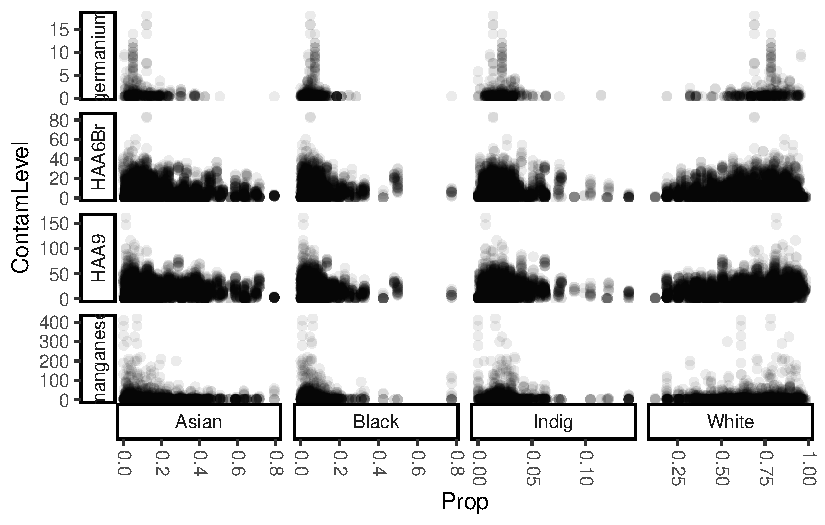
\includegraphics{appendix_files/figure-pdf/plotting contams and race/eth-1.pdf}

\hypertarget{deciding-models-and-checking-assumptions}{%
\subsection{Deciding models and checking
assumptions}\label{deciding-models-and-checking-assumptions}}

\hypertarget{germanium}{%
\paragraph{Germanium}\label{germanium}}

\hypertarget{deciding-model}{%
\subparagraph{Deciding model}\label{deciding-model}}

\begin{Shaded}
\begin{Highlighting}[]
\NormalTok{germanium }\OtherTok{\textless{}{-}}\NormalTok{ full }\SpecialCharTok{\%\textgreater{}\%} 
  \FunctionTok{filter}\NormalTok{(Contaminant }\SpecialCharTok{==} \StringTok{"germanium"}\NormalTok{)}

\CommentTok{\# race}
\NormalTok{germanium\_gamma }\OtherTok{\textless{}{-}} \FunctionTok{glm}\NormalTok{(ContamLevel }\SpecialCharTok{\textasciitilde{}}\NormalTok{ Prop }\SpecialCharTok{*}\NormalTok{ RaceEth, }\AttributeTok{data =}\NormalTok{ germanium, }\AttributeTok{family =}\NormalTok{ Gamma)}
\NormalTok{germanium\_lm }\OtherTok{\textless{}{-}} \FunctionTok{glm}\NormalTok{(ContamLevel }\SpecialCharTok{\textasciitilde{}}\NormalTok{ Prop }\SpecialCharTok{*}\NormalTok{ RaceEth, }\AttributeTok{data =}\NormalTok{ germanium)}
\NormalTok{germanium\_log }\OtherTok{\textless{}{-}} \FunctionTok{glm}\NormalTok{(LogLevel }\SpecialCharTok{\textasciitilde{}}\NormalTok{ Prop }\SpecialCharTok{*}\NormalTok{ RaceEth, }\AttributeTok{data =}\NormalTok{ germanium)}

\NormalTok{rcompanion}\SpecialCharTok{::}\FunctionTok{compareGLM}\NormalTok{(germanium\_gamma, germanium\_lm) }\CommentTok{\# gamma wins!}
\end{Highlighting}
\end{Shaded}

\begin{verbatim}
$Models
  Formula                       
1 "ContamLevel ~ Prop * RaceEth"
2 "ContamLevel ~ Prop * RaceEth"

$Fit.criteria
  Rank Df.res  AIC AICc  BIC McFadden Cox.and.Snell Nagelkerke   p.value
1    8   2120 5560 5560 5611 0.016190       0.04194    0.04514 1.331e-18
2    8   2120 9829 9829 9880 0.002459       0.01130    0.01141 5.282e-28
\end{verbatim}

\begin{Shaded}
\begin{Highlighting}[]
\NormalTok{rcompanion}\SpecialCharTok{::}\FunctionTok{compareGLM}\NormalTok{(germanium\_gamma, germanium\_log) }\CommentTok{\# log{-}transformed y wins!}
\end{Highlighting}
\end{Shaded}

\begin{verbatim}
$Models
  Formula                       
1 "ContamLevel ~ Prop * RaceEth"
2 "LogLevel ~ Prop * RaceEth"   

$Fit.criteria
  Rank Df.res  AIC AICc  BIC McFadden Cox.and.Snell Nagelkerke   p.value
1    8   2120 5560 5560 5611  0.01619       0.04194    0.04514 1.331e-18
2    8   2120 2179 2179 2230  0.01989       0.02040    0.03162 1.016e-01
\end{verbatim}

\begin{Shaded}
\begin{Highlighting}[]
\CommentTok{\# ethnicity}
\NormalTok{germanium\_lm\_eth }\OtherTok{\textless{}{-}} \FunctionTok{glm}\NormalTok{(ContamLevel }\SpecialCharTok{\textasciitilde{}}\NormalTok{ HispLat\_prop, }\AttributeTok{data =}\NormalTok{ germanium)}
\NormalTok{germanium\_log\_eth }\OtherTok{\textless{}{-}} \FunctionTok{glm}\NormalTok{(LogLevel }\SpecialCharTok{\textasciitilde{}}\NormalTok{ HispLat\_prop, }\AttributeTok{data =}\NormalTok{ germanium)}

\NormalTok{rcompanion}\SpecialCharTok{::}\FunctionTok{compareGLM}\NormalTok{(germanium\_lm\_eth, germanium\_log\_eth) }\CommentTok{\# log{-}transformed y wins!}
\end{Highlighting}
\end{Shaded}

\begin{verbatim}
$Models
  Formula                     
1 "ContamLevel ~ HispLat_prop"
2 "LogLevel ~ HispLat_prop"   

$Fit.criteria
  Rank Df.res  AIC AICc  BIC McFadden Cox.and.Snell Nagelkerke   p.value
1    2   2126 9799 9799 9816 0.004302       0.01968    0.01988 1.770e-56
2    2   2126 2188 2189 2205 0.010260       0.01058    0.01639 3.231e-02
\end{verbatim}

Since smaller AIC, BIC, p-value and larger McFadden are all evidence of
a better fit, we choose the model with a log-transformed response
variable.

\hypertarget{checking-assumptions}{%
\subparagraph{Checking assumptions}\label{checking-assumptions}}

\begin{Shaded}
\begin{Highlighting}[]
\FunctionTok{plot}\NormalTok{(germanium\_log) }\CommentTok{\# log{-}transformed contaminant levels}
\end{Highlighting}
\end{Shaded}

\begin{figure}[H]

{\centering 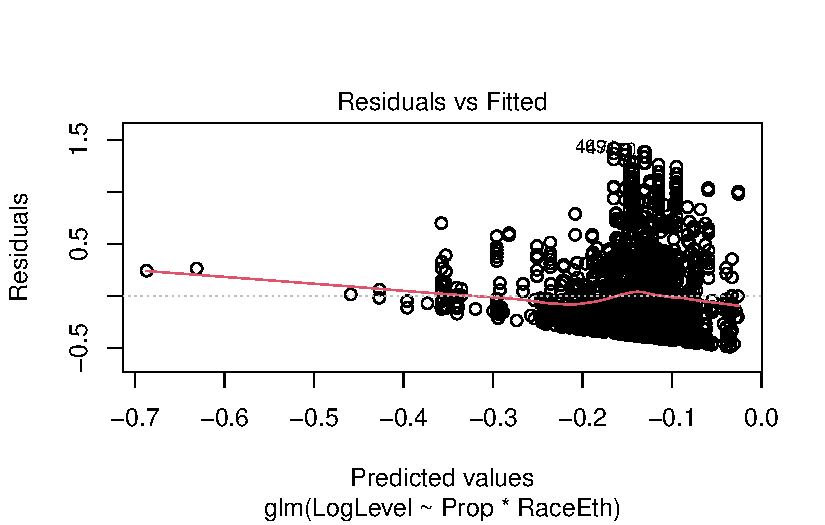
\includegraphics[width=0.5\textwidth,height=\textheight]{appendix_files/figure-pdf/unnamed-chunk-3-1.pdf}

}

\end{figure}

\begin{figure}[H]

{\centering 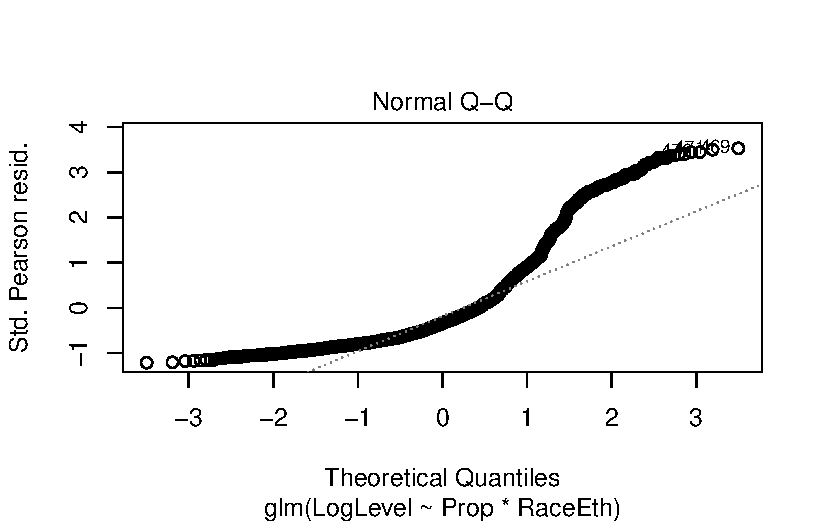
\includegraphics[width=0.5\textwidth,height=\textheight]{appendix_files/figure-pdf/unnamed-chunk-3-2.pdf}

}

\end{figure}

\begin{figure}[H]

{\centering 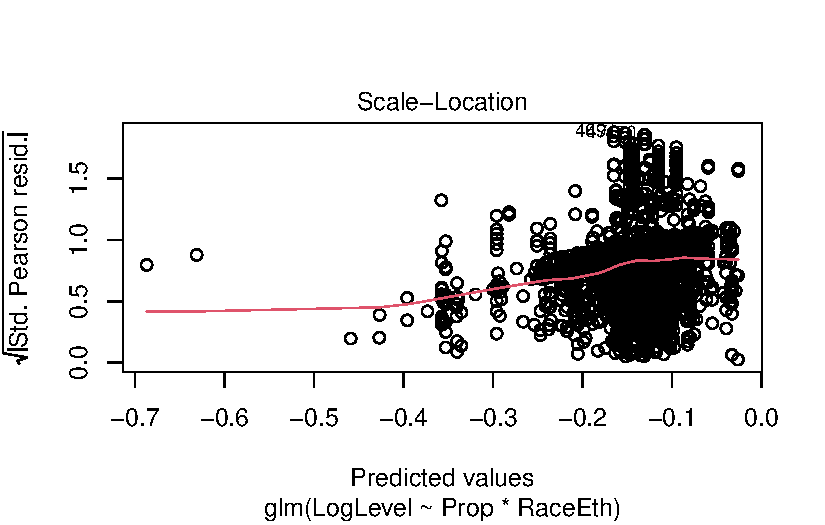
\includegraphics[width=0.5\textwidth,height=\textheight]{appendix_files/figure-pdf/unnamed-chunk-3-3.pdf}

}

\end{figure}

\begin{figure}[H]

{\centering 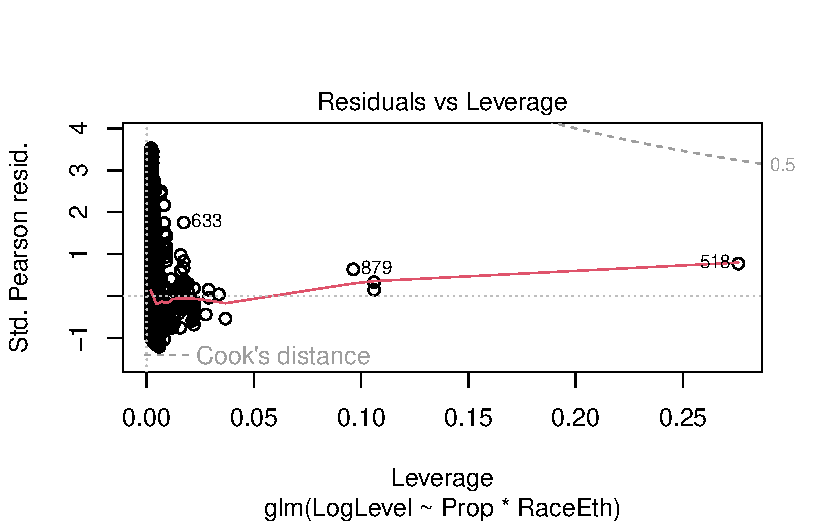
\includegraphics[width=0.5\textwidth,height=\textheight]{appendix_files/figure-pdf/unnamed-chunk-3-4.pdf}

}

\end{figure}

\hypertarget{manganese}{%
\paragraph{Manganese}\label{manganese}}

\begin{Shaded}
\begin{Highlighting}[]
\NormalTok{manganese }\OtherTok{\textless{}{-}}\NormalTok{ full }\SpecialCharTok{\%\textgreater{}\%}
  \FunctionTok{filter}\NormalTok{(Contaminant }\SpecialCharTok{==} \StringTok{"manganese"}\NormalTok{)}

\CommentTok{\# race}
\NormalTok{manganese\_gamma }\OtherTok{\textless{}{-}} \FunctionTok{glm}\NormalTok{(ContamLevel }\SpecialCharTok{\textasciitilde{}}\NormalTok{ Prop }\SpecialCharTok{*}\NormalTok{ RaceEth, }\AttributeTok{data =}\NormalTok{ manganese, }\AttributeTok{family =}\NormalTok{ Gamma)}
\NormalTok{manganese\_lm }\OtherTok{\textless{}{-}} \FunctionTok{glm}\NormalTok{(ContamLevel }\SpecialCharTok{\textasciitilde{}}\NormalTok{ Prop }\SpecialCharTok{*}\NormalTok{ RaceEth, }\AttributeTok{data =}\NormalTok{ manganese)}
\NormalTok{manganese\_log }\OtherTok{\textless{}{-}} \FunctionTok{glm}\NormalTok{(LogLevel }\SpecialCharTok{\textasciitilde{}}\NormalTok{ Prop }\SpecialCharTok{*}\NormalTok{ RaceEth, }\AttributeTok{data =}\NormalTok{ manganese)}

\NormalTok{rcompanion}\SpecialCharTok{::}\FunctionTok{compareGLM}\NormalTok{(manganese\_gamma, manganese\_lm) }\CommentTok{\# gamma wins!}
\end{Highlighting}
\end{Shaded}

\begin{verbatim}
$Models
  Formula                       
1 "ContamLevel ~ Prop * RaceEth"
2 "ContamLevel ~ Prop * RaceEth"

$Fit.criteria
  Rank Df.res    AIC   AICc    BIC  McFadden Cox.and.Snell Nagelkerke   p.value
1    8  14240  83540  83540  83610 0.0023350      0.013630   0.013670 1.918e-74
2    8  14240 132900 132900 133000 0.0002095      0.001953   0.001953 0.000e+00
\end{verbatim}

\begin{Shaded}
\begin{Highlighting}[]
\NormalTok{rcompanion}\SpecialCharTok{::}\FunctionTok{compareGLM}\NormalTok{(manganese\_gamma, manganese\_log) }\CommentTok{\# log{-}transformed y wins!}
\end{Highlighting}
\end{Shaded}

\begin{verbatim}
$Models
  Formula                       
1 "ContamLevel ~ Prop * RaceEth"
2 "LogLevel ~ Prop * RaceEth"   

$Fit.criteria
  Rank Df.res   AIC  AICc   BIC  McFadden Cox.and.Snell Nagelkerke   p.value
1    8  14240 83540 83540 83610 0.0023350     0.0136300    0.01367 1.918e-74
2    8  14240 24710 24710 24780 0.0005132     0.0008896    0.00108 1.178e-01
\end{verbatim}

\begin{Shaded}
\begin{Highlighting}[]
\FunctionTok{plot}\NormalTok{(manganese\_log)}

\CommentTok{\# ethnicity}
\NormalTok{manganese\_lm\_eth }\OtherTok{\textless{}{-}} \FunctionTok{glm}\NormalTok{(ContamLevel }\SpecialCharTok{\textasciitilde{}}\NormalTok{ HispLat\_prop, }\AttributeTok{data =}\NormalTok{ manganese)}
\NormalTok{manganese\_log\_eth }\OtherTok{\textless{}{-}} \FunctionTok{glm}\NormalTok{(LogLevel }\SpecialCharTok{\textasciitilde{}}\NormalTok{ HispLat\_prop, }\AttributeTok{data =}\NormalTok{ manganese)}

\NormalTok{rcompanion}\SpecialCharTok{::}\FunctionTok{compareGLM}\NormalTok{(manganese\_lm\_eth, manganese\_log\_eth) }\CommentTok{\# log{-}transformed y wins!}
\end{Highlighting}
\end{Shaded}

\begin{verbatim}
$Models
  Formula                     
1 "ContamLevel ~ HispLat_prop"
2 "LogLevel ~ HispLat_prop"   

$Fit.criteria
  Rank Df.res    AIC   AICc    BIC  McFadden Cox.and.Snell Nagelkerke  p.value
1    2  14240 132900 132900 132900 0.0004683      0.004360   0.004361 0.000000
2    2  14240  24680  24680  24700 0.0010880      0.001885   0.002289 0.001558
\end{verbatim}

\begin{Shaded}
\begin{Highlighting}[]
\FunctionTok{plot}\NormalTok{(manganese\_log\_eth)}
\end{Highlighting}
\end{Shaded}

\begin{figure}[H]

{\centering 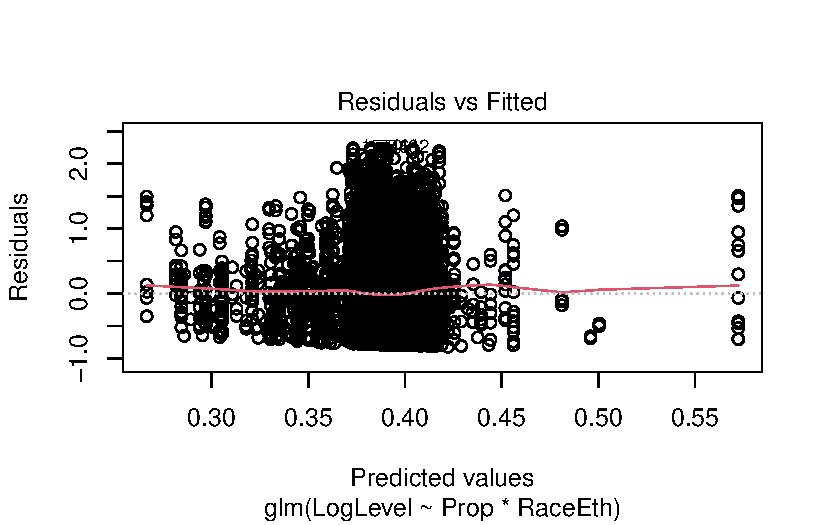
\includegraphics[width=0.5\textwidth,height=\textheight]{appendix_files/figure-pdf/unnamed-chunk-4-1.pdf}

}

\end{figure}

\begin{figure}[H]

{\centering 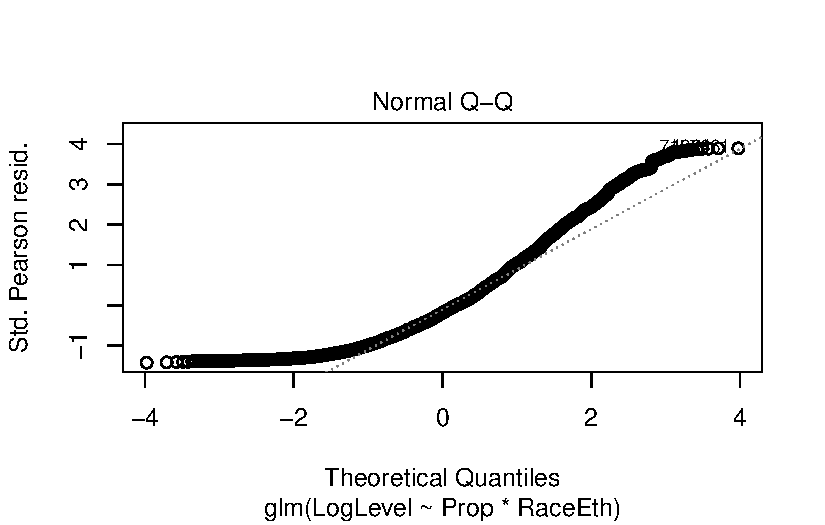
\includegraphics[width=0.5\textwidth,height=\textheight]{appendix_files/figure-pdf/unnamed-chunk-4-2.pdf}

}

\end{figure}

\begin{figure}[H]

{\centering 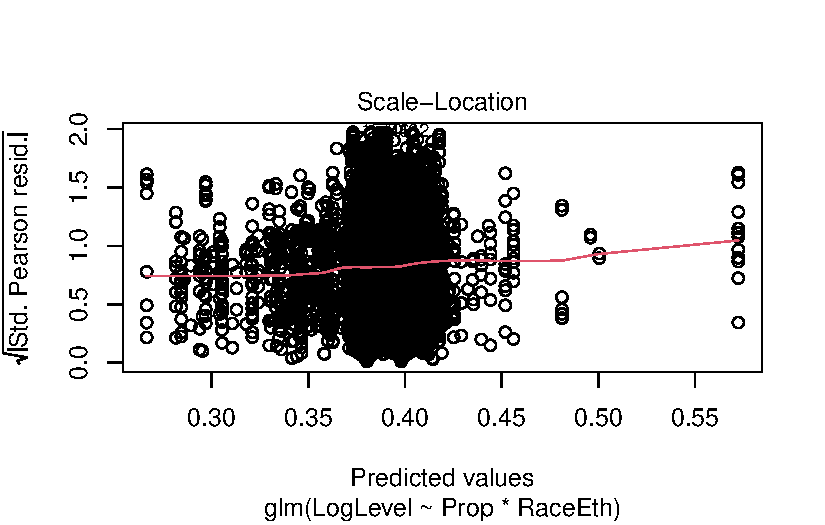
\includegraphics[width=0.5\textwidth,height=\textheight]{appendix_files/figure-pdf/unnamed-chunk-4-3.pdf}

}

\end{figure}

\begin{figure}[H]

{\centering 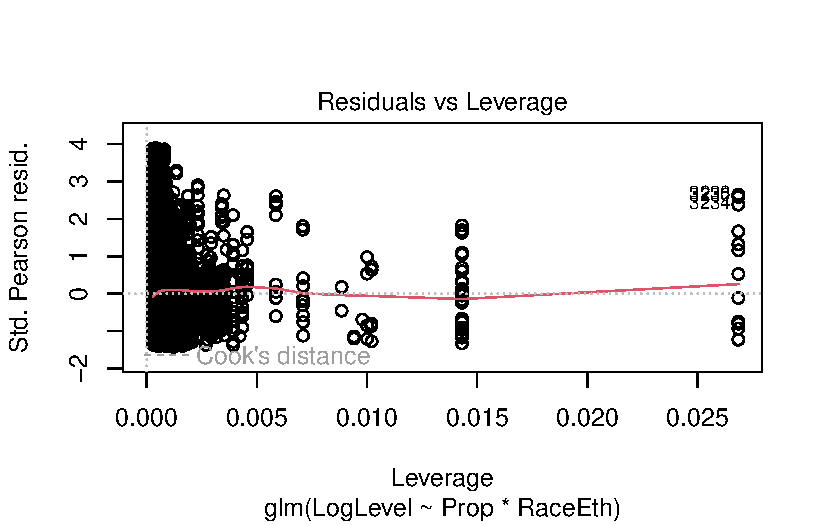
\includegraphics[width=0.5\textwidth,height=\textheight]{appendix_files/figure-pdf/unnamed-chunk-4-4.pdf}

}

\end{figure}

\begin{figure}[H]

{\centering 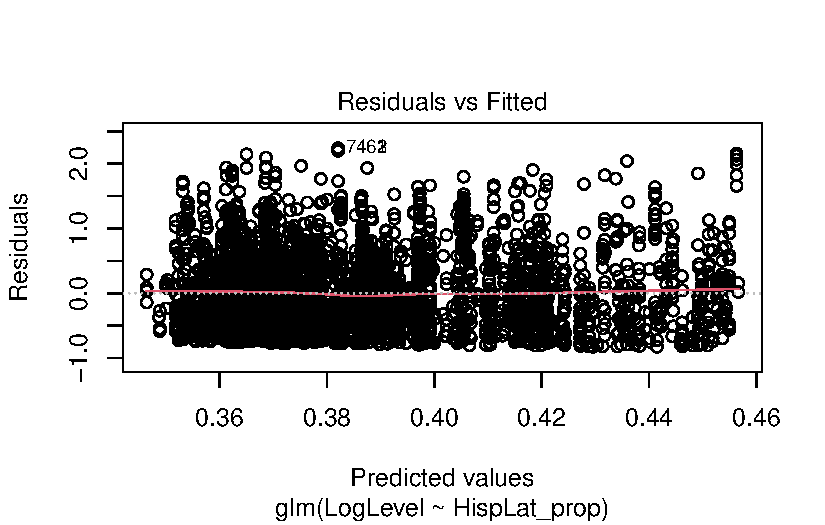
\includegraphics[width=0.5\textwidth,height=\textheight]{appendix_files/figure-pdf/unnamed-chunk-4-5.pdf}

}

\end{figure}

\begin{figure}[H]

{\centering 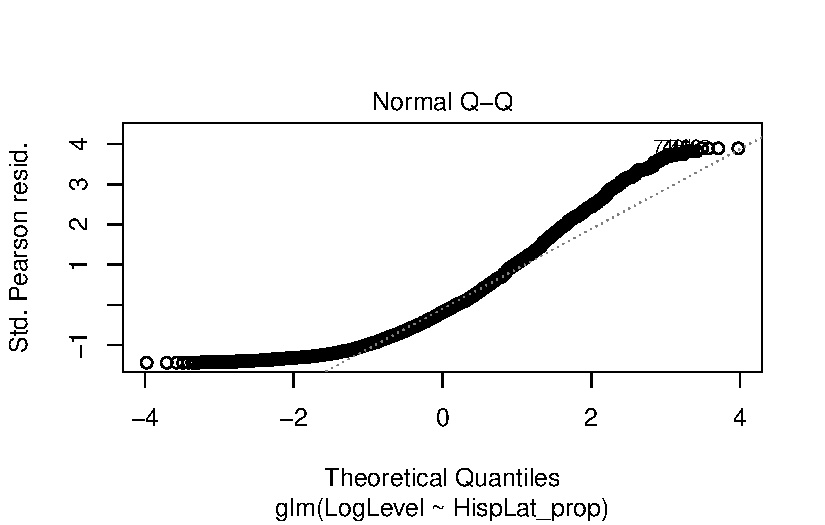
\includegraphics[width=0.5\textwidth,height=\textheight]{appendix_files/figure-pdf/unnamed-chunk-4-6.pdf}

}

\end{figure}

\begin{figure}[H]

{\centering 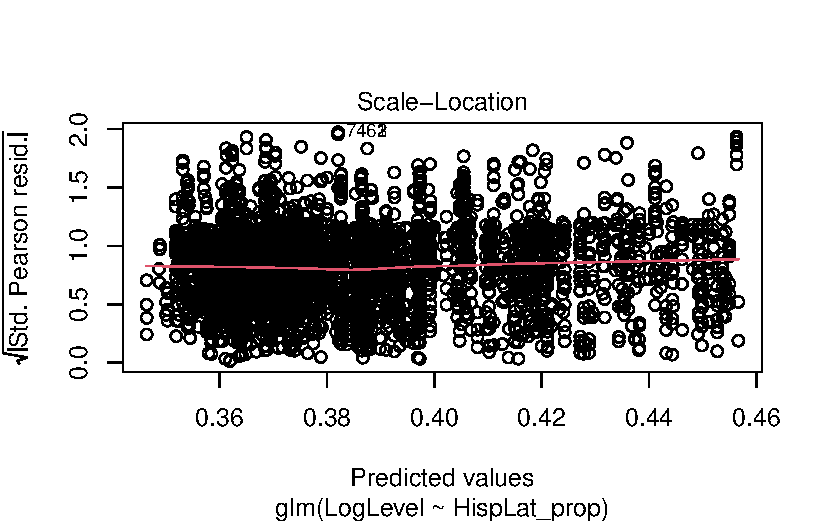
\includegraphics[width=0.5\textwidth,height=\textheight]{appendix_files/figure-pdf/unnamed-chunk-4-7.pdf}

}

\end{figure}

\begin{figure}[H]

{\centering 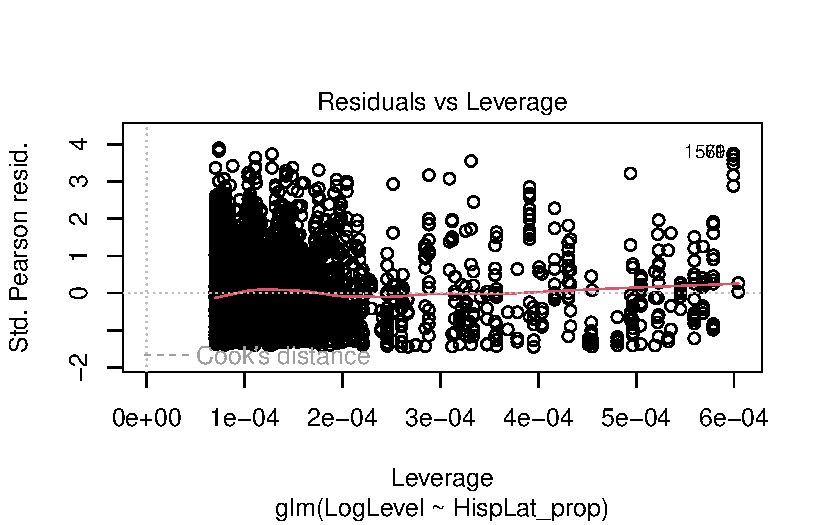
\includegraphics[width=0.5\textwidth,height=\textheight]{appendix_files/figure-pdf/unnamed-chunk-4-8.pdf}

}

\end{figure}

\hypertarget{haa6br}{%
\paragraph{HAA6Br}\label{haa6br}}

\begin{Shaded}
\begin{Highlighting}[]
\NormalTok{HAA6Br }\OtherTok{\textless{}{-}}\NormalTok{ full }\SpecialCharTok{\%\textgreater{}\%} 
  \FunctionTok{filter}\NormalTok{(Contaminant }\SpecialCharTok{==} \StringTok{"HAA6Br"}\NormalTok{)}

\CommentTok{\# race}
\NormalTok{HAA6Br\_gamma }\OtherTok{\textless{}{-}} \FunctionTok{glm}\NormalTok{(ContamLevel }\SpecialCharTok{\textasciitilde{}}\NormalTok{ Prop }\SpecialCharTok{*}\NormalTok{ RaceEth, }\AttributeTok{data =}\NormalTok{ HAA6Br, }\AttributeTok{family =}\NormalTok{ Gamma)}
\NormalTok{HAA6Br\_lm }\OtherTok{\textless{}{-}} \FunctionTok{glm}\NormalTok{(ContamLevel }\SpecialCharTok{\textasciitilde{}}\NormalTok{ Prop }\SpecialCharTok{*}\NormalTok{ RaceEth, }\AttributeTok{data =}\NormalTok{ HAA6Br)}
\NormalTok{HAA6Br\_log }\OtherTok{\textless{}{-}} \FunctionTok{glm}\NormalTok{(LogLevel }\SpecialCharTok{\textasciitilde{}}\NormalTok{ Prop }\SpecialCharTok{*}\NormalTok{ RaceEth, }\AttributeTok{data =}\NormalTok{ HAA6Br)}

\NormalTok{rcompanion}\SpecialCharTok{::}\FunctionTok{compareGLM}\NormalTok{(HAA6Br\_gamma, HAA6Br\_lm) }\CommentTok{\# gamma wins!}
\end{Highlighting}
\end{Shaded}

\begin{verbatim}
$Models
  Formula                       
1 "ContamLevel ~ Prop * RaceEth"
2 "ContamLevel ~ Prop * RaceEth"

$Fit.criteria
  Rank Df.res    AIC   AICc    BIC  McFadden Cox.and.Snell Nagelkerke   p.value
1    8  29200 175500 175500 175600 0.0011230      0.006734   0.006750 1.607e-38
2    8  29200 200200 200200 200200 0.0008801      0.006017   0.006023 0.000e+00
\end{verbatim}

\begin{Shaded}
\begin{Highlighting}[]
\NormalTok{rcompanion}\SpecialCharTok{::}\FunctionTok{compareGLM}\NormalTok{(HAA6Br\_gamma, HAA6Br\_log) }\CommentTok{\# log{-}transformed y wins!}
\end{Highlighting}
\end{Shaded}

\begin{verbatim}
$Models
  Formula                       
1 "ContamLevel ~ Prop * RaceEth"
2 "LogLevel ~ Prop * RaceEth"   

$Fit.criteria
  Rank Df.res    AIC   AICc    BIC McFadden Cox.and.Snell Nagelkerke   p.value
1    8  29200 175500 175500 175600 0.001123      0.006734   0.006750 1.607e-38
2    8  29200  44830  44830  44900 0.004349      0.006678   0.008499 1.460e-09
\end{verbatim}

\begin{Shaded}
\begin{Highlighting}[]
\FunctionTok{plot}\NormalTok{(HAA6Br\_log)}

\CommentTok{\# ethnicity}
\NormalTok{HAA6Br\_lm\_eth }\OtherTok{\textless{}{-}} \FunctionTok{glm}\NormalTok{(ContamLevel }\SpecialCharTok{\textasciitilde{}}\NormalTok{ HispLat\_prop, }\AttributeTok{data =}\NormalTok{ HAA6Br)}
\NormalTok{HAA6Br\_log\_eth }\OtherTok{\textless{}{-}} \FunctionTok{glm}\NormalTok{(LogLevel }\SpecialCharTok{\textasciitilde{}}\NormalTok{ HispLat\_prop, }\AttributeTok{data =}\NormalTok{ HAA6Br)}

\NormalTok{rcompanion}\SpecialCharTok{::}\FunctionTok{compareGLM}\NormalTok{(HAA6Br\_lm\_eth, HAA6Br\_log\_eth) }\CommentTok{\# log{-}transformed y wins!}
\end{Highlighting}
\end{Shaded}

\begin{verbatim}
$Models
  Formula                     
1 "ContamLevel ~ HispLat_prop"
2 "LogLevel ~ HispLat_prop"   

$Fit.criteria
  Rank Df.res    AIC   AICc    BIC  McFadden Cox.and.Snell Nagelkerke p.value
1    2  29210 200300 200300 200300 0.0003199     0.0021910  0.0021930  0.0000
2    2  29210  45010  45010  45030 0.0000825     0.0001271  0.0001618  0.2385
\end{verbatim}

\begin{Shaded}
\begin{Highlighting}[]
\FunctionTok{plot}\NormalTok{(HAA6Br\_log\_eth)}
\end{Highlighting}
\end{Shaded}

\begin{figure}[H]

{\centering 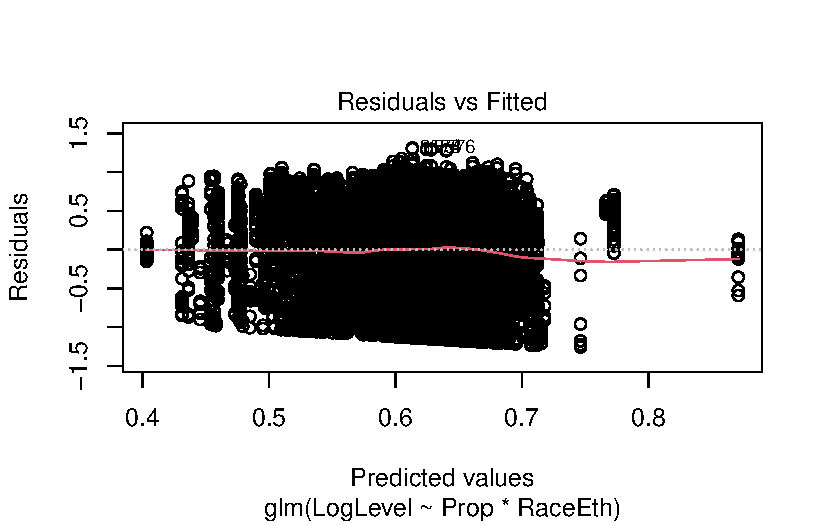
\includegraphics[width=0.5\textwidth,height=\textheight]{appendix_files/figure-pdf/unnamed-chunk-5-1.pdf}

}

\end{figure}

\begin{figure}[H]

{\centering 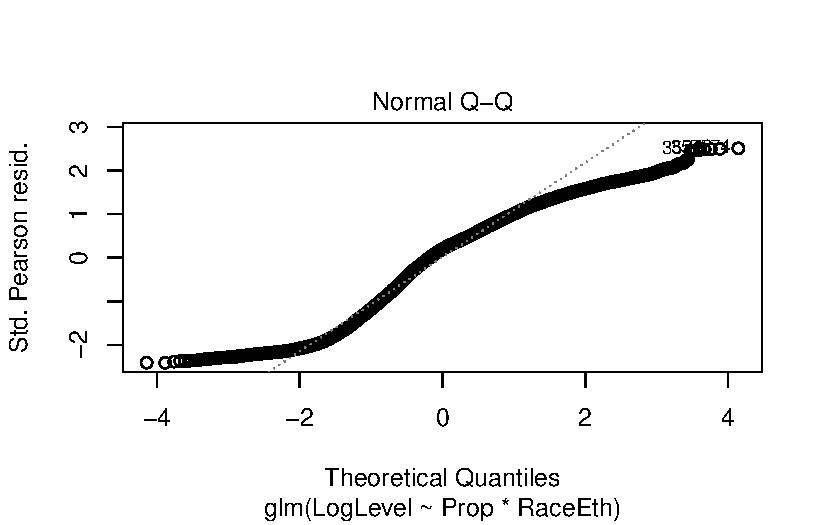
\includegraphics[width=0.5\textwidth,height=\textheight]{appendix_files/figure-pdf/unnamed-chunk-5-2.pdf}

}

\end{figure}

\begin{figure}[H]

{\centering 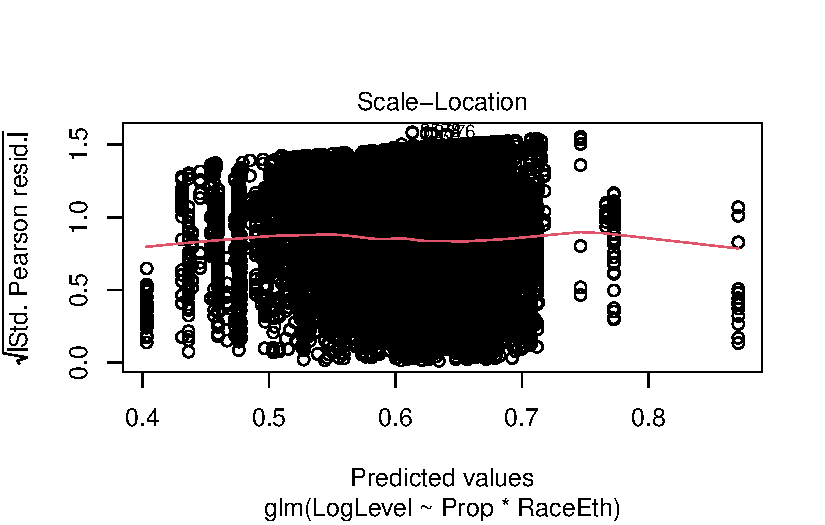
\includegraphics[width=0.5\textwidth,height=\textheight]{appendix_files/figure-pdf/unnamed-chunk-5-3.pdf}

}

\end{figure}

\begin{figure}[H]

{\centering 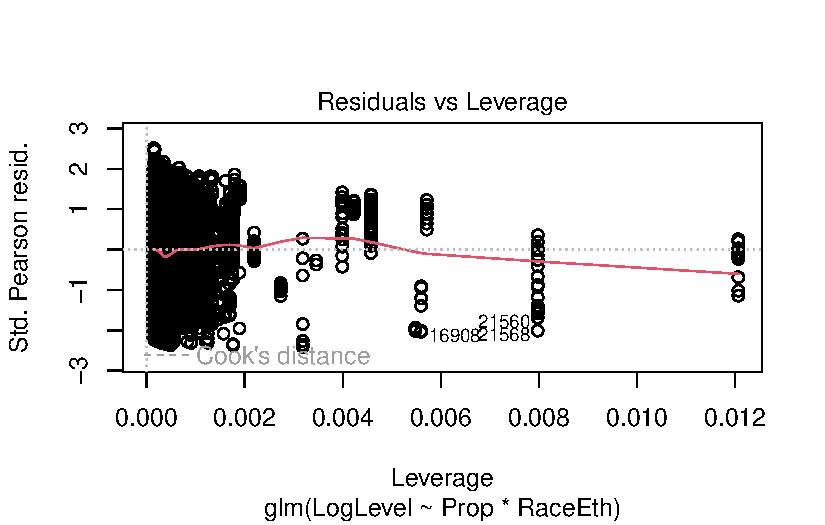
\includegraphics[width=0.5\textwidth,height=\textheight]{appendix_files/figure-pdf/unnamed-chunk-5-4.pdf}

}

\end{figure}

\begin{figure}[H]

{\centering 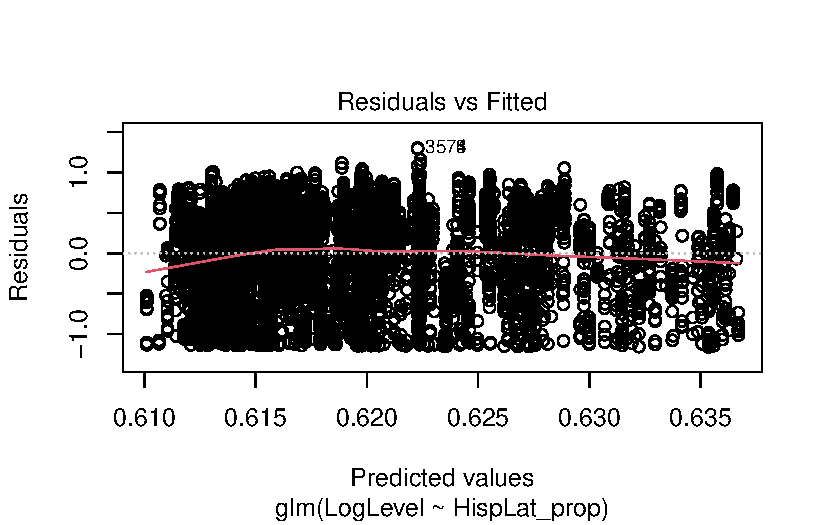
\includegraphics[width=0.5\textwidth,height=\textheight]{appendix_files/figure-pdf/unnamed-chunk-5-5.pdf}

}

\end{figure}

\begin{figure}[H]

{\centering 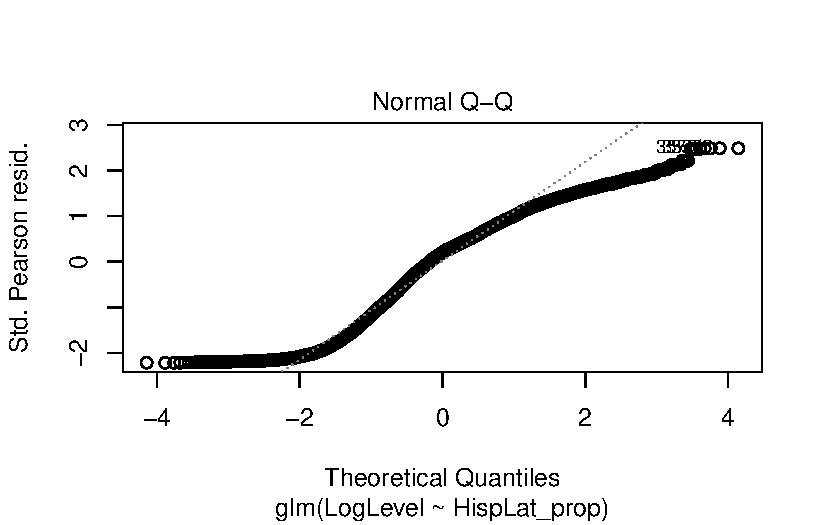
\includegraphics[width=0.5\textwidth,height=\textheight]{appendix_files/figure-pdf/unnamed-chunk-5-6.pdf}

}

\end{figure}

\begin{figure}[H]

{\centering 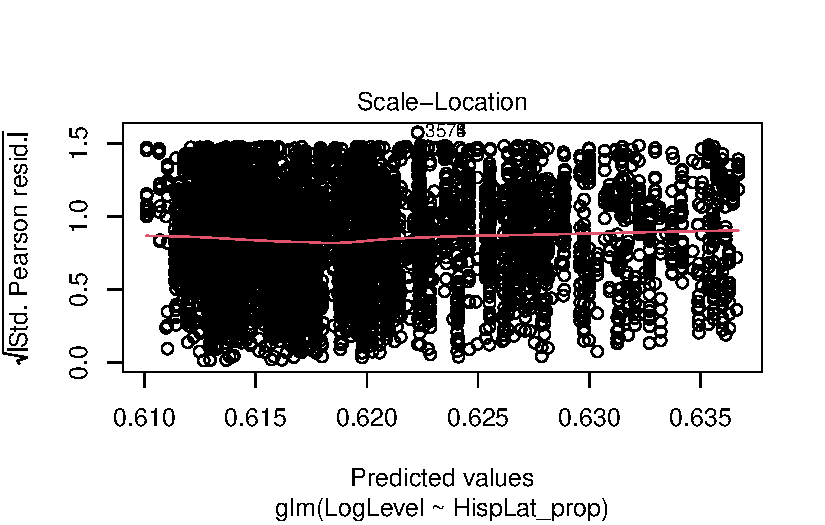
\includegraphics[width=0.5\textwidth,height=\textheight]{appendix_files/figure-pdf/unnamed-chunk-5-7.pdf}

}

\end{figure}

\begin{figure}[H]

{\centering 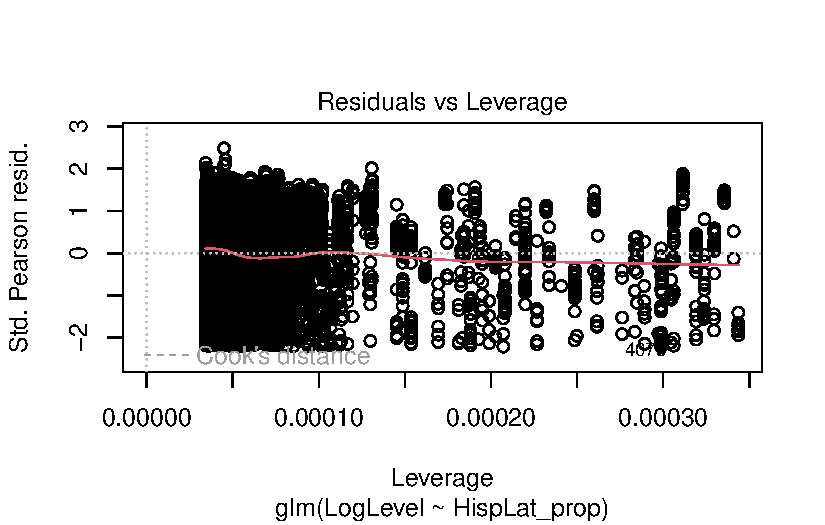
\includegraphics[width=0.5\textwidth,height=\textheight]{appendix_files/figure-pdf/unnamed-chunk-5-8.pdf}

}

\end{figure}

\hypertarget{haa9}{%
\paragraph{HAA9}\label{haa9}}

\begin{Shaded}
\begin{Highlighting}[]
\NormalTok{HAA9 }\OtherTok{\textless{}{-}}\NormalTok{ full }\SpecialCharTok{\%\textgreater{}\%} 
  \FunctionTok{filter}\NormalTok{(Contaminant }\SpecialCharTok{==} \StringTok{"HAA9"}\NormalTok{)}

\CommentTok{\# race}
\NormalTok{HAA9\_gamma }\OtherTok{\textless{}{-}} \FunctionTok{glm}\NormalTok{(ContamLevel }\SpecialCharTok{\textasciitilde{}}\NormalTok{ Prop }\SpecialCharTok{*}\NormalTok{ RaceEth, }\AttributeTok{data =}\NormalTok{ HAA9, }\AttributeTok{family =}\NormalTok{ Gamma)}
\NormalTok{HAA9\_lm }\OtherTok{\textless{}{-}} \FunctionTok{glm}\NormalTok{(ContamLevel }\SpecialCharTok{\textasciitilde{}}\NormalTok{ Prop }\SpecialCharTok{*}\NormalTok{ RaceEth, }\AttributeTok{data =}\NormalTok{ HAA9)}
\NormalTok{HAA9\_log }\OtherTok{\textless{}{-}} \FunctionTok{glm}\NormalTok{(LogLevel }\SpecialCharTok{\textasciitilde{}}\NormalTok{ Prop }\SpecialCharTok{*}\NormalTok{ RaceEth, }\AttributeTok{data =}\NormalTok{ HAA9)}

\NormalTok{rcompanion}\SpecialCharTok{::}\FunctionTok{compareGLM}\NormalTok{(HAA9\_gamma, HAA9\_lm) }\CommentTok{\# gamma wins!}
\end{Highlighting}
\end{Shaded}

\begin{verbatim}
$Models
  Formula                       
1 "ContamLevel ~ Prop * RaceEth"
2 "ContamLevel ~ Prop * RaceEth"

$Fit.criteria
  Rank Df.res    AIC   AICc    BIC  McFadden Cox.and.Snell Nagelkerke p.value
1    8  30080 231400 231400 231500 0.0007617      0.005845   0.005848 4.2e-30
2    8  30080 245000 245000 245100 0.0008797      0.007143   0.007145 0.0e+00
\end{verbatim}

\begin{Shaded}
\begin{Highlighting}[]
\NormalTok{rcompanion}\SpecialCharTok{::}\FunctionTok{compareGLM}\NormalTok{(HAA9\_gamma, HAA9\_log) }\CommentTok{\# log{-}transformed y wins!}
\end{Highlighting}
\end{Shaded}

\begin{verbatim}
$Models
  Formula                       
1 "ContamLevel ~ Prop * RaceEth"
2 "LogLevel ~ Prop * RaceEth"   

$Fit.criteria
  Rank Df.res    AIC   AICc    BIC  McFadden Cox.and.Snell Nagelkerke   p.value
1    8  30080 231400 231400 231500 0.0007617      0.005845   0.005848 4.200e-30
2    8  30080  47830  47830  47910 0.0041960      0.006675   0.008372 1.723e-10
\end{verbatim}

\begin{Shaded}
\begin{Highlighting}[]
\FunctionTok{plot}\NormalTok{(HAA9\_log)}

\CommentTok{\# ethnicity}
\NormalTok{HAA9\_lm\_eth }\OtherTok{\textless{}{-}} \FunctionTok{glm}\NormalTok{(ContamLevel }\SpecialCharTok{\textasciitilde{}}\NormalTok{ HispLat\_prop, }\AttributeTok{data =}\NormalTok{ HAA9)}
\NormalTok{HAA9\_log\_eth }\OtherTok{\textless{}{-}} \FunctionTok{glm}\NormalTok{(LogLevel }\SpecialCharTok{\textasciitilde{}}\NormalTok{ HispLat\_prop, }\AttributeTok{data =}\NormalTok{ HAA9)}

\NormalTok{rcompanion}\SpecialCharTok{::}\FunctionTok{compareGLM}\NormalTok{(HAA9\_lm\_eth, HAA9\_log\_eth) }\CommentTok{\# log{-}transformed y wins!}
\end{Highlighting}
\end{Shaded}

\begin{verbatim}
$Models
  Formula                     
1 "ContamLevel ~ HispLat_prop"
2 "LogLevel ~ HispLat_prop"   

$Fit.criteria
  Rank Df.res    AIC   AICc    BIC McFadden Cox.and.Snell Nagelkerke    p.value
1    2  30080 244300 244300 244300  0.00349       0.02804    0.02805  0.000e+00
2    2  30080  46010  46010  46040  0.04187       0.06465    0.08108 1.678e-124
\end{verbatim}

\begin{Shaded}
\begin{Highlighting}[]
\FunctionTok{plot}\NormalTok{(HAA9\_log\_eth)}
\end{Highlighting}
\end{Shaded}

\begin{figure}[H]

{\centering 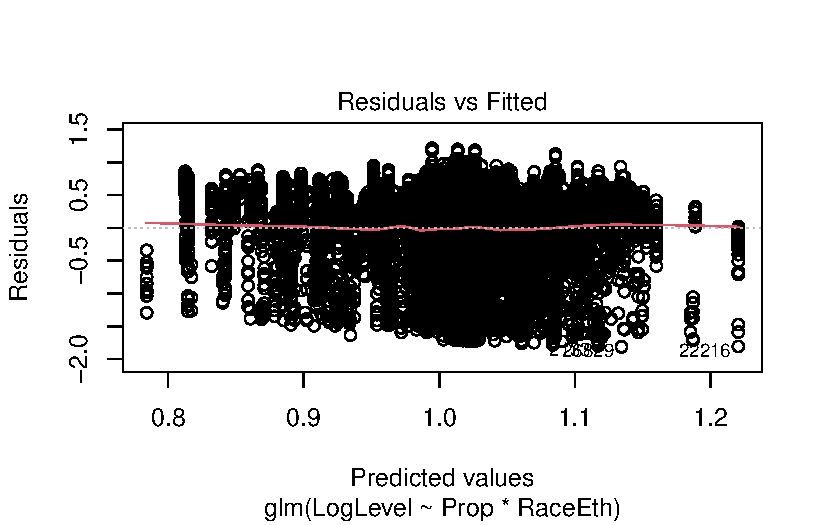
\includegraphics[width=0.5\textwidth,height=\textheight]{appendix_files/figure-pdf/unnamed-chunk-6-1.pdf}

}

\end{figure}

\begin{figure}[H]

{\centering 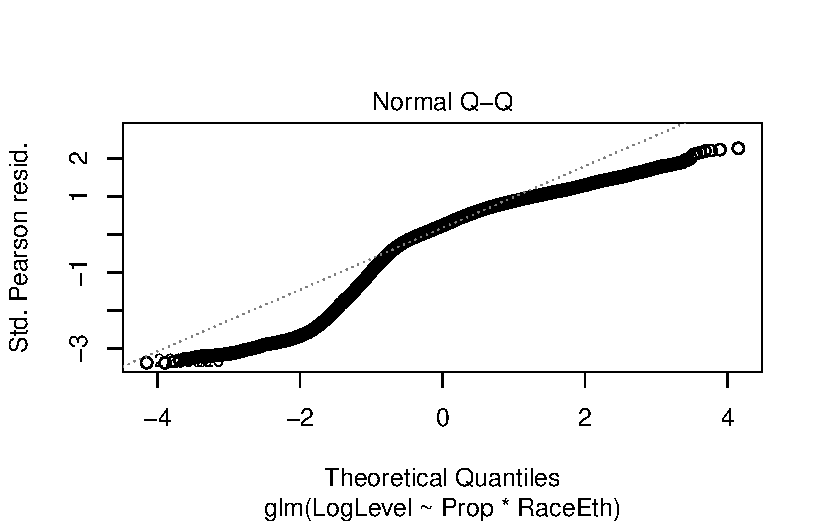
\includegraphics[width=0.5\textwidth,height=\textheight]{appendix_files/figure-pdf/unnamed-chunk-6-2.pdf}

}

\end{figure}

\begin{figure}[H]

{\centering 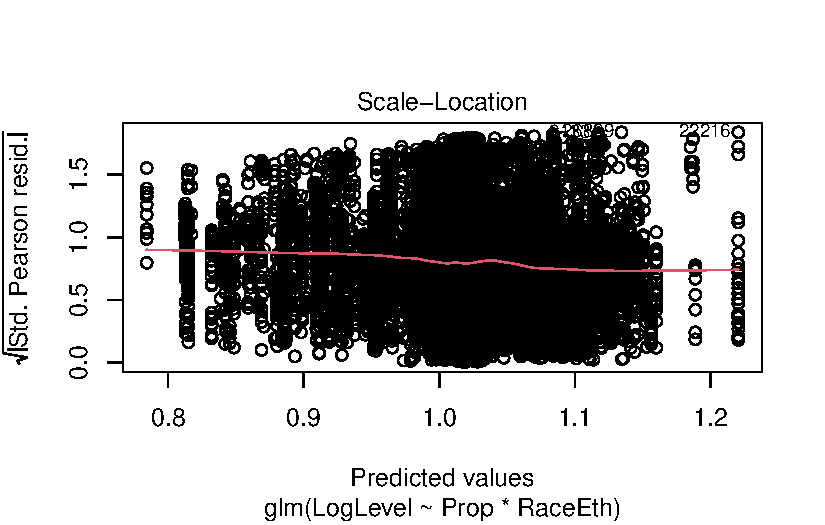
\includegraphics[width=0.5\textwidth,height=\textheight]{appendix_files/figure-pdf/unnamed-chunk-6-3.pdf}

}

\end{figure}

\begin{figure}[H]

{\centering 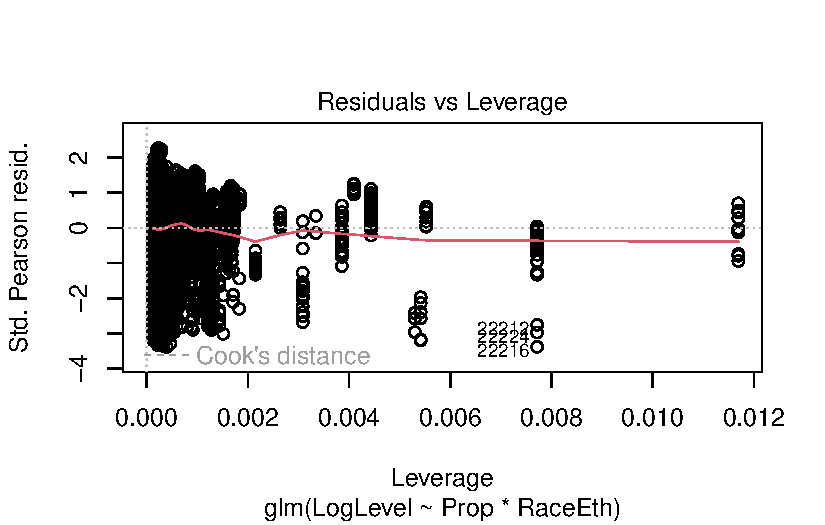
\includegraphics[width=0.5\textwidth,height=\textheight]{appendix_files/figure-pdf/unnamed-chunk-6-4.pdf}

}

\end{figure}

\begin{figure}[H]

{\centering 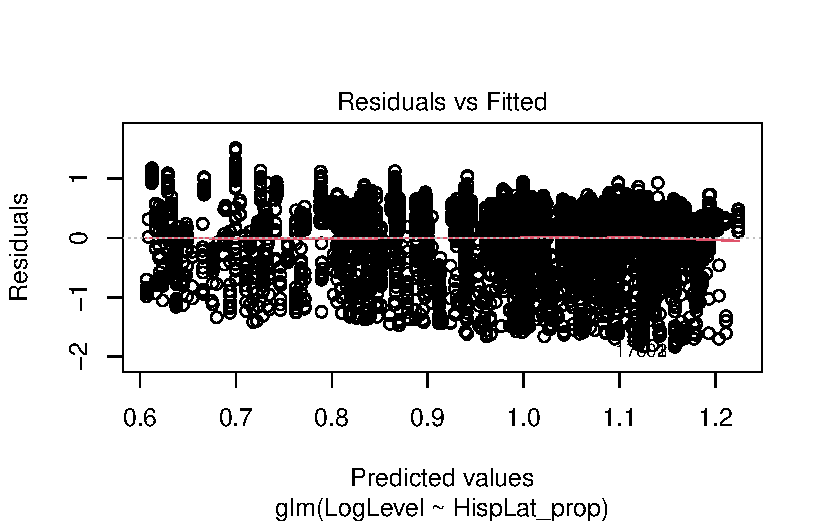
\includegraphics[width=0.5\textwidth,height=\textheight]{appendix_files/figure-pdf/unnamed-chunk-6-5.pdf}

}

\end{figure}

\begin{figure}[H]

{\centering 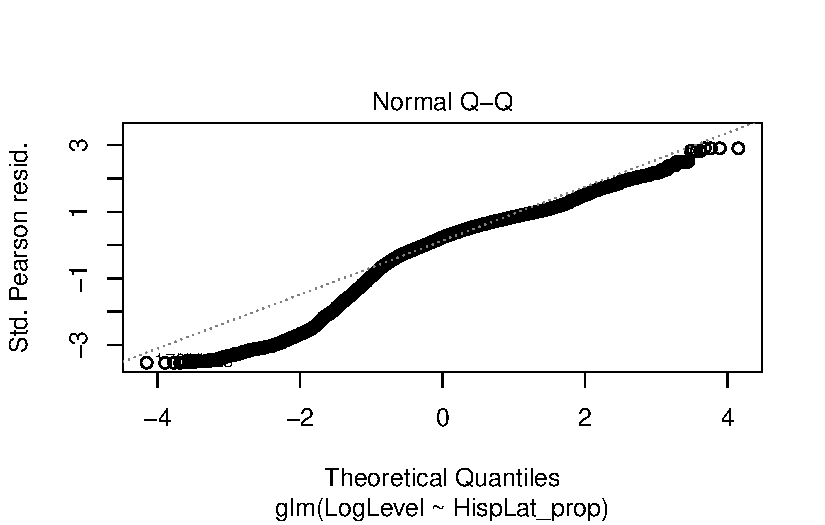
\includegraphics[width=0.5\textwidth,height=\textheight]{appendix_files/figure-pdf/unnamed-chunk-6-6.pdf}

}

\end{figure}

\begin{figure}[H]

{\centering 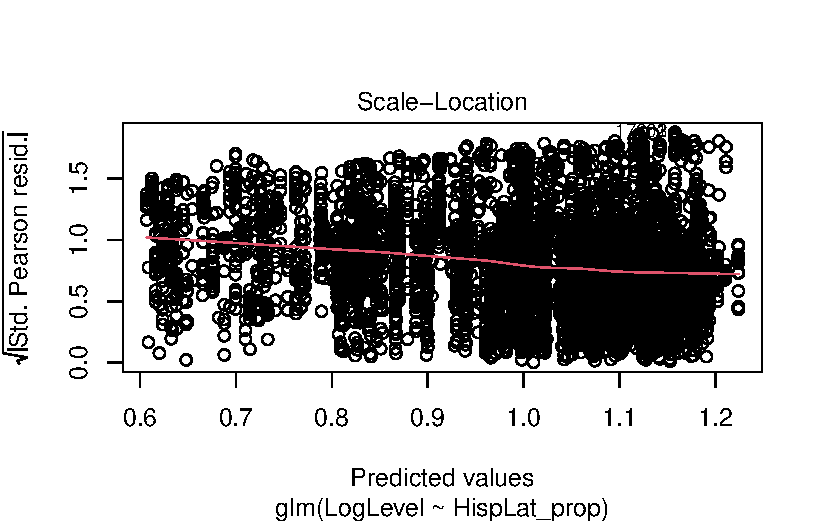
\includegraphics[width=0.5\textwidth,height=\textheight]{appendix_files/figure-pdf/unnamed-chunk-6-7.pdf}

}

\end{figure}

\begin{figure}[H]

{\centering 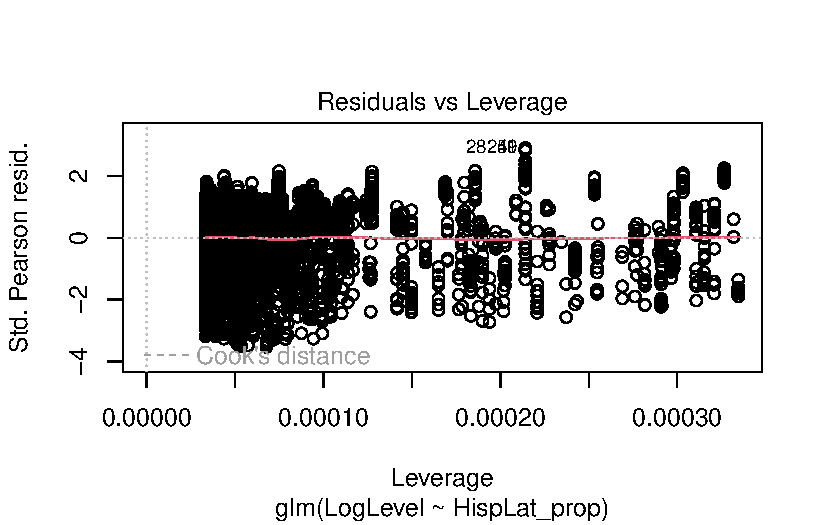
\includegraphics[width=0.5\textwidth,height=\textheight]{appendix_files/figure-pdf/unnamed-chunk-6-8.pdf}

}

\end{figure}



\end{document}
